\chapter{Implementation}
This chapter describes the implementation of GeoDude and some of the considerations aswell as the functionality.

\section{GPS module}
The knowledge about pin assignments for the GPS module, RGM-2000, comes from the website: \url{http://www.tobias-schlegel.de/?page_id=51&lang=en}.\\ 
The communication settings were found in the User Manual (RGM-2000\_user\_manual.pdf which can be found in appendix):\\
\begin{table}[H]
    \begin{tabular}{|ll|}
    \hline
    Baud rate    & : 4800 \\ \hline
    Data bit     & : 8    \\ \hline
    Parity       & : None \\ \hline
    Stop bit     & : 1    \\ \hline
    Flow control & : None \\ \hline
    \end{tabular}
\end{table}
To understand the format output from the GPS module, NMEA-0183, we consulted the wikipedia site as well as observing on Tx in RealTerm (terminal software). The raw NMEA-0183 string looks like this:\\
\begin{verbatim}
$GPGGA,092750.000,5321.6802,N,00630.3372,W,1,8,1.03,61.7,M,55.2,M,,*76
\end{verbatim}
To display this data in an understandable way, we have to cut the string up and "send" it. 

\section{Screen}
The screen is a nokia 3310 display controlled by a PCD8544. The PCD8544 has an SPI interface along with three control pins. These pins are: Chip enable, reset and data/command pin.\\
The data/command pin is used to tell the display whether a command or data has been transmitted. Below a figure from the datasheet is displayed, showing how a transmission should be done.

\begin{figure}[hbpt]
\centering
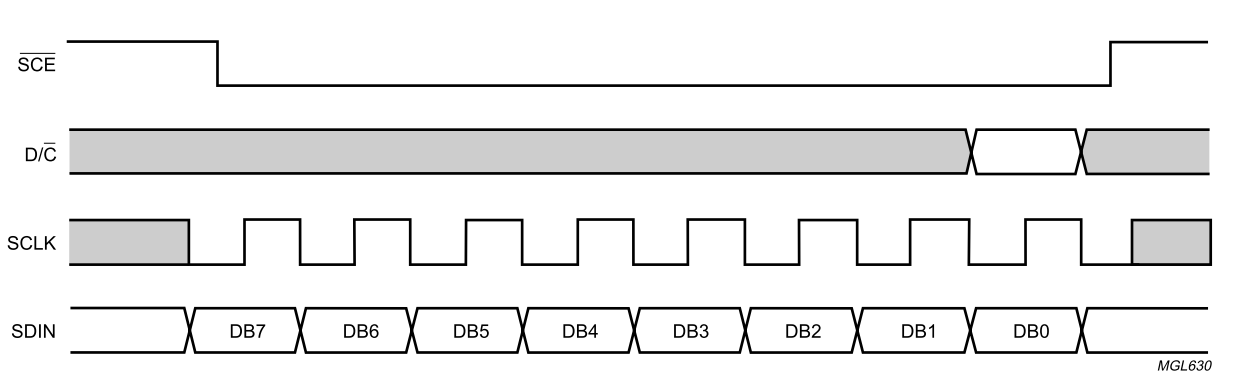
\includegraphics[width=.8\textwidth]{billeder/Display_protocol}
\end{figure}
Commands to the display is used for setup purposes such as contrast, cursor position, ram addressing etc. Data to the display is used to set the pixels to either on or off. The display is divided into "banks" where a bank consists of 8 pixels. It has 6 banks in height and 84 banks in width.\\


\section{Magnetometer}
The magnetometer is a HMC6352 and is interfaced using i$^2$c.

\section{Software structure}
The software implemented in this project is described by the UML diagram in the figure below.\\
The system is described via. UML even though it is made in C it offers a nice overview of all headers, variables and function calls.
\begin{figure}[hbpt]
\centering
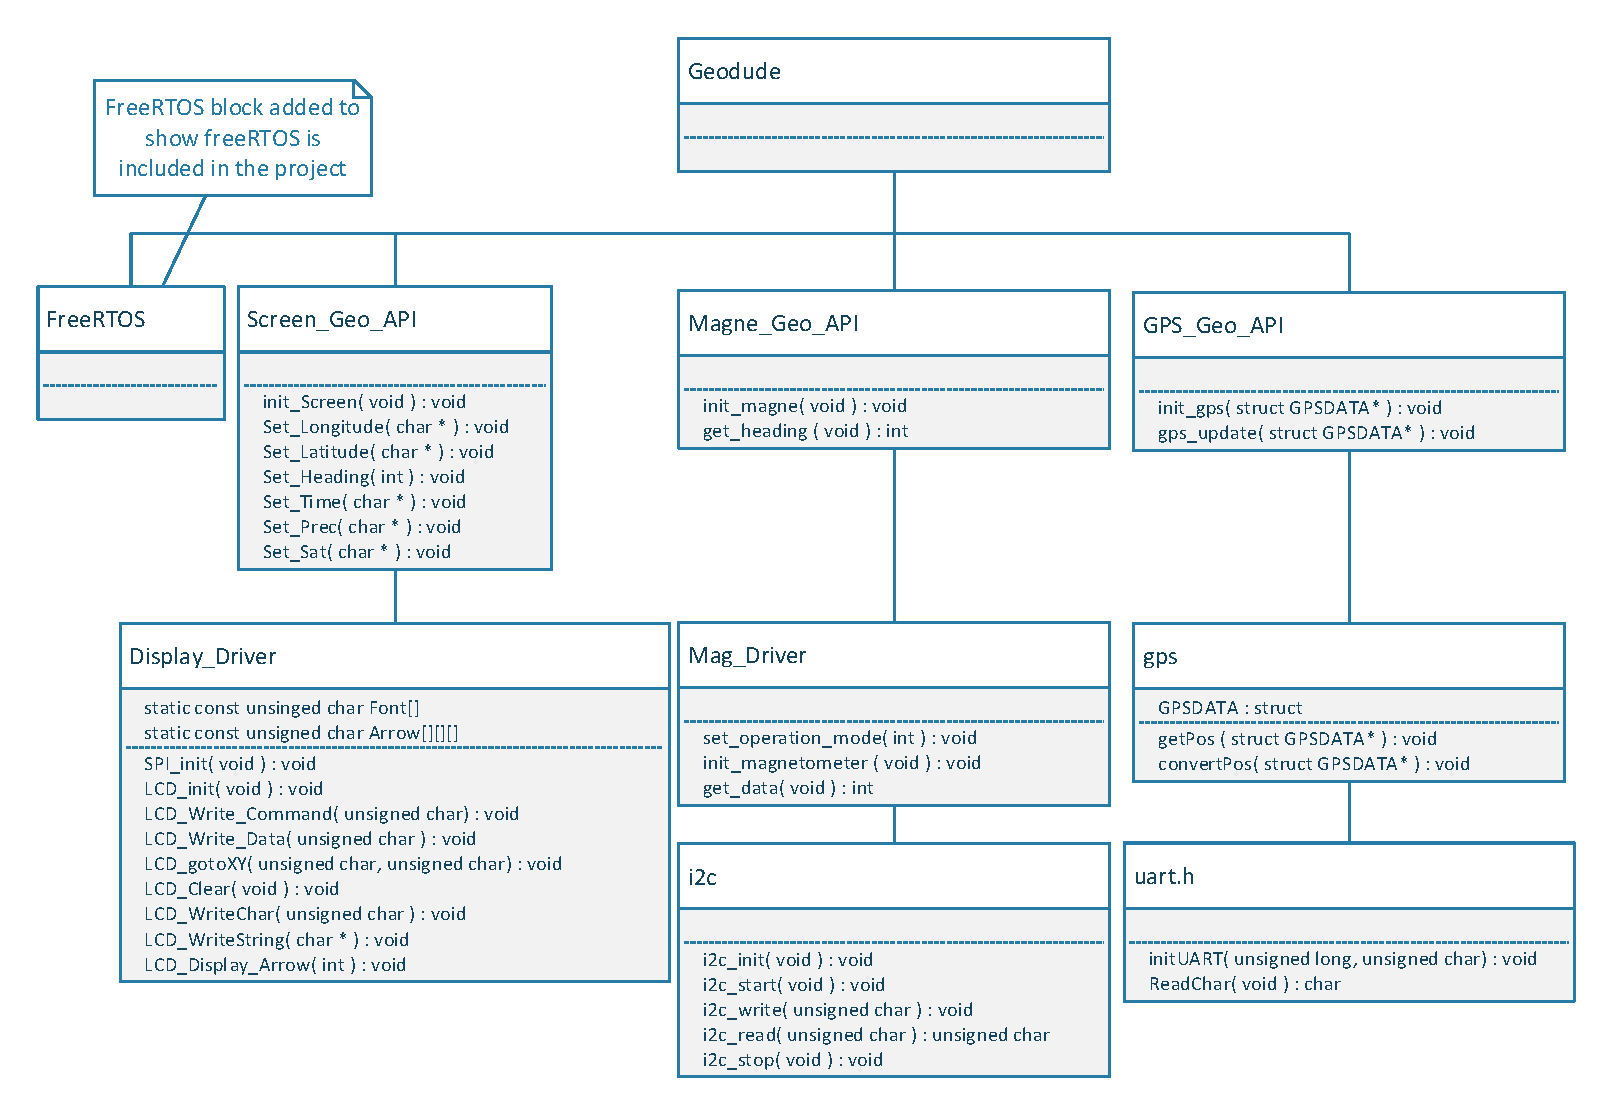
\includegraphics[width=1\textwidth]{billeder/geodude_UML}
\caption{Geodude UML diagram}
\end{figure}